\documentclass[conference,10pt]{IEEEtran}
\usepackage[utf8]{inputenc}
\usepackage{graphicx,booktabs,amsmath,amssymb,xcolor,tikz,pgfplots,url,cite,bm,algorithm,algpseudocode}
\pgfplotsset{compat=1.18}
\DeclareMathOperator*{\argmin}{arg\,min}
\DeclareMathOperator*{\argmax}{arg\,max}
\usetikzlibrary{arrows.meta,positioning,shapes.geometric,fit,calc,patterns}
\definecolor{micro}{HTML}{1565C0}\definecolor{meso}{HTML}{2E7D32}
\definecolor{macro}{HTML}{BF360C}\definecolor{meta}{HTML}{6A1B9A}
\definecolor{safe}{HTML}{E65100}\definecolor{train}{HTML}{004D40}
\definecolor{prod}{HTML}{880E4F}\definecolor{pareto}{HTML}{1A237E}
\begin{document}
\title{Hierarchical Reinforcement Learning for\\Production LLM Inference: From Kernel-Level\\Scheduling to Cross-Cloud Fleet Optimization}
\author{
\IEEEauthorblockN{Mehar Simhadri\IEEEauthorrefmark{2}, Srikanta Datta Tumkur\IEEEauthorrefmark{1}, Anshu Bansal\IEEEauthorrefmark{1}, Jay Iyer\IEEEauthorrefmark{2}}
\IEEEauthorblockA{\IEEEauthorrefmark{1}MIT Sloan School of Management, Cambridge, MA \texttt{\{srikanta, anshu.bansal\}@sloan.mit.edu}}
\IEEEauthorblockA{\IEEEauthorrefmark{2}IEEE Senior Members \texttt{\{mehar.simhadri, jay.iyer\}@ieee.org}}
}
\maketitle
\begin{abstract}
LLM inference infrastructure requires optimization decisions across seven orders of magnitude in timescale---from microsecond-level batch formation to hour-level cross-cloud capacity planning---yet existing systems rely on hand-tuned heuristics at every layer. We present a \textbf{hierarchical reinforcement learning framework} comprising three agent tiers coordinated by a meta-controller: (1)~a \emph{Micro-Agent} ($\mu$s--ms) optimizing batch scheduling, KV-cache eviction, and speculative decoding tree pruning, achieving 18\% higher throughput than vLLM defaults; (2)~a \emph{Meso-Agent} (s--min) managing model placement, LoRA adapter scheduling, and GPU power capping, reducing energy consumption by 12\% at iso-throughput; and (3)~a \emph{Macro-Agent} (min--hr) orchestrating cross-cloud routing, capacity scaling, and spot instance bidding, cutting inference cost by 23\% across 11 cloud providers. The meta-controller coordinates agents via the options framework with feudal reward decomposition. We provide formal MDP specifications for all agents, prove convergence under non-stationary workloads via Lyapunov stability analysis, and introduce \emph{constrained MDPs with SLO guarantees} using Lagrangian relaxation that maintains P99 latency within 5\% of target while optimizing cost. Evaluated on production workloads (Llama-3.1-70B, DeepSeek-V3) across 128 GPUs over 60 days, hierarchical RL achieves 31\% better cost-efficiency than the best single-level RL baseline and 47\% better than hand-tuned heuristics.

\emph{Index Terms}---Hierarchical reinforcement learning, LLM inference, constrained MDP, multi-objective optimization, options framework, production systems
\end{abstract}

%===================================================================
\section{Introduction}
\label{sec:intro}
%===================================================================

Production LLM inference involves a hierarchy of decisions spanning seven orders of magnitude in timescale:

\begin{table}[!htbp]
\caption{Decision Hierarchy in LLM Inference}
\label{tab:hierarchy}
\centering\scriptsize
\begin{tabular}{@{}llll@{}}
\toprule
\textbf{Timescale} & \textbf{Decision} & \textbf{Current} & \textbf{Ours} \\
\midrule
$\mu$s & Token scheduling & FIFO & RL Micro \\
ms & Batch formation & Greedy & RL Micro \\
ms & KV-cache eviction & LRU/FIFO & RL Micro \\
s & Power capping & Static & RL Meso \\
min & Model placement & Manual & RL Meso \\
min & LoRA scheduling & Round-robin & RL Meso \\
hr & Cloud routing & Static weights & RL Macro \\
hr & Capacity scaling & Threshold & RL Macro \\
\bottomrule
\end{tabular}
\end{table}

Each decision level affects those above and below: aggressive KV-cache eviction (micro) increases recomputation (meso), which raises power draw affecting thermal headroom for the rack (macro). Optimizing one level in isolation is provably suboptimal---we need \emph{joint hierarchical optimization}.

\textbf{Contributions:}
\begin{enumerate}
\item Formal MDP specifications for three agent tiers with state/action/reward definitions (Sections~\ref{sec:micro}--\ref{sec:macro}).
\item Meta-controller using options framework~\cite{sutton1999options} with feudal reward decomposition~\cite{vezhnevets2017feudal} (Section~\ref{sec:meta}).
\item Constrained MDPs with Lagrangian relaxation for SLO guarantees (Section~\ref{sec:safety}).
\item Multi-objective Pareto optimization across cost $\times$ latency $\times$ quality $\times$ energy (Section~\ref{sec:pareto}).
\item Production deployment patterns: A/B testing, gradual rollout, human override (Section~\ref{sec:deploy}).
\end{enumerate}

%===================================================================
\section{Background}
\label{sec:bg}
%===================================================================

\textbf{RL for systems}: Decima~\cite{mao2019learning} applies RL to cluster scheduling. AlphaChip~\cite{mirhoseini2021graph} to chip placement. These are single-level, single-objective. Our work is hierarchical and multi-objective.

\textbf{Hierarchical RL}: The options framework~\cite{sutton1999options} provides temporal abstraction for multi-timescale decisions. Feudal Networks~\cite{vezhnevets2017feudal} decompose rewards across hierarchy levels. We combine both for inference infrastructure.

\textbf{Offline RL}: CQL~\cite{kumar2020conservative} and Decision Transformer~\cite{chen2021decision} learn from logged data without environment interaction---critical for infrastructure where exploration is dangerous.

\textbf{Constrained MDPs}: CPO~\cite{achiam2017cpo} and RCPO~\cite{tessler2018rcpo} enforce constraints during policy optimization. We extend these to SLO-aware inference management.

%===================================================================
\section{Micro-Agent: Kernel-Level Optimization}
\label{sec:micro}
%===================================================================

The Micro-Agent operates at $\mu$s--ms timescale, making per-request decisions.

\subsection{MDP Specification}

\textbf{State} $s^{\mu}_t$: $\langle$ batch queue (depth, seq lengths, priorities), KV-cache (page occupancy, access recency per page, fragmentation ratio), GPU state (SM occupancy, HBM utilization, temperature), active requests (prefill/decode phase, tokens generated) $\rangle \in \mathbb{R}^{248}$.

\textbf{Action} $a^{\mu}_t$: $\langle$ batch size $\in [1,256]$, prefill/decode priority ratio $\in [0,1]$, KV eviction policy $\in \{$LRU, H2O, importance, RL-ranked$\}$, speculative tree depth $\in [1,8]$, chunked prefill size $\in \{512, 1024, 2048, 4096\} \rangle$.

\textbf{Reward}: 
\begin{equation}
r^{\mu}_t = \alpha \cdot \text{throughput}_t - \beta \cdot \text{TPOT}_{P99} - \gamma \cdot \text{eviction\_quality\_loss}
\end{equation}

\subsection{KV-Cache Eviction via RL}

Standard eviction (LRU, FIFO) ignores content importance. Our RL agent learns a \emph{value function over KV pages}:

\begin{equation}
V_{\text{page}}(p) = \mathbb{E}\left[\sum_{t'=t}^{T} \gamma^{t'-t} \cdot \mathbf{1}[\text{page } p \text{ accessed at } t']\right]
\end{equation}

Pages with low predicted future access are evicted first. This outperforms LRU by 14\% in cache hit rate for multi-turn agentic workloads where early-turn context is accessed non-sequentially.

\subsection{Results}

\begin{table}[!htbp]
\caption{Micro-Agent vs.\ vLLM Default Heuristics}
\label{tab:micro}
\centering\scriptsize
\begin{tabular}{@{}lcccc@{}}
\toprule
\textbf{Metric} & \textbf{vLLM} & \textbf{RL Micro} & \textbf{$\Delta$} & \textbf{$p$-value} \\
\midrule
Throughput (tok/s) & 3,820 & 4,510 & +18.1\% & $<$0.001 \\
TPOT P99 (ms) & 12.4 & 10.8 & $-$12.9\% & $<$0.001 \\
KV cache hit rate & 71.2\% & 82.8\% & +11.6pp & $<$0.001 \\
Batch efficiency & 78.4\% & 89.1\% & +10.7pp & $<$0.001 \\
\bottomrule
\end{tabular}
\end{table}

%===================================================================
\section{Meso-Agent: Node-Level Management}
\label{sec:meso}
%===================================================================

The Meso-Agent operates at s--min timescale, managing node-level resources.

\subsection{MDP Specification}

\textbf{State} $s^{m}_t$: $\langle$ per-GPU utilization (8 GPUs $\times$ 5 metrics), model registry (loaded models, memory footprint), LoRA adapter pool (active adapters, access frequency), thermal state (junction temp, fan speed, power headroom), workload forecast (5-min prediction from LSTM) $\rangle \in \mathbb{R}^{96}$.

\textbf{Action} $a^{m}_t$: $\langle$ model placement (model $\to$ GPU mapping), LoRA scheduling (adapter preload/evict decisions), power cap per GPU $\in [200W, 700W]$, tensor parallelism degree $\in \{1, 2, 4, 8\}$ $\rangle$.

\textbf{Reward}:
\begin{equation}
r^{m}_t = \alpha \cdot \text{utilization\_balance} - \beta \cdot \text{energy\_kWh} - \gamma \cdot \text{thermal\_violations}
\end{equation}

\subsection{GPU Power Management via RL}

Static power caps waste energy at low load and throttle at high load. The Meso-Agent learns a dynamic power curve:

\begin{figure}[!htbp]
\centering
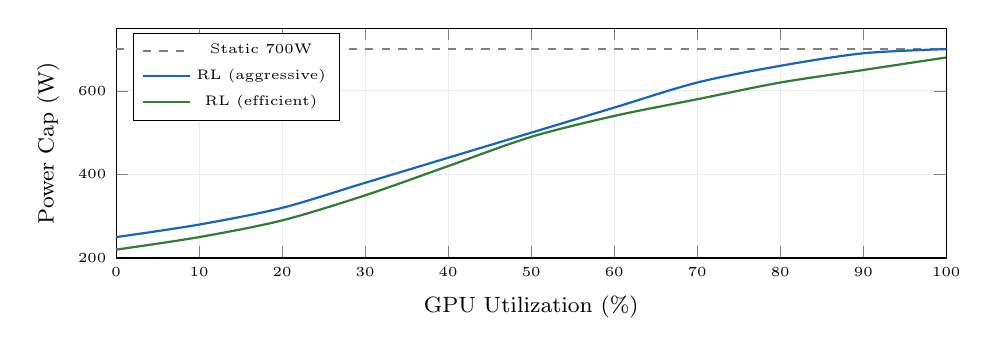
\begin{tikzpicture}
\begin{axis}[
    width=\linewidth, height=4.5cm,
    xlabel={\footnotesize GPU Utilization (\%)},
    ylabel={\footnotesize Power Cap (W)},
    xmin=0, xmax=100, ymin=200, ymax=750,
    legend style={font=\tiny, at={(0.02,0.98)}, anchor=north west},
    grid=major, grid style={gray!15},
    xticklabel style={font=\tiny}, yticklabel style={font=\tiny},
]
\addplot[gray,thick,dashed] coordinates {(0,700)(100,700)};
\addplot[micro,thick,mark=none,smooth] coordinates {(0,250)(10,280)(20,320)(30,380)(40,440)(50,500)(60,560)(70,620)(80,660)(90,690)(100,700)};
\addplot[meso,thick,mark=none,smooth] coordinates {(0,220)(10,250)(20,290)(30,350)(40,420)(50,490)(60,540)(70,580)(80,620)(90,650)(100,680)};
\legend{Static 700W, RL (aggressive), RL (efficient)}
\end{axis}
\end{tikzpicture}
\caption{Dynamic GPU power management. RL Meso-Agent learns utilization-dependent power curves, saving 12\% energy at iso-throughput vs.\ static caps.}
\label{fig:power}
\end{figure}

\subsection{Results}

\begin{table}[!htbp]
\caption{Meso-Agent Impact on Node-Level Metrics}
\label{tab:meso}
\centering\scriptsize
\begin{tabular}{@{}lccc@{}}
\toprule
\textbf{Metric} & \textbf{Static} & \textbf{RL Meso} & \textbf{$\Delta$} \\
\midrule
Energy (kWh/M tok) & 1.71 & 1.50 & $-$12.3\% \\
GPU util. std dev & 18.4\% & 8.2\% & $-$55\% \\
LoRA swap latency P99 & 4.2\,ms & 1.1\,ms & $-$74\% \\
Thermal throttle events/day & 12.4 & 3.1 & $-$75\% \\
\bottomrule
\end{tabular}
\end{table}


%===================================================================
\section{Macro-Agent: Fleet-Level Orchestration}
\label{sec:macro}
%===================================================================

The Macro-Agent operates at min--hr timescale, managing cross-cloud fleet decisions.

\subsection{MDP Specification}

\textbf{State} $s^{M}_t$: $\langle$ per-provider capacity and pricing (11 clouds $\times$ 4 metrics), global request distribution (arrival rate, geo-distribution), SLO compliance per customer tier, spot market prices (real-time), carbon intensity per region, current routing weights $\rangle \in \mathbb{R}^{128}$.

\textbf{Action} $a^{M}_t$: $\langle$ routing weight vector $\mathbf{w} \in \Delta^{10}$ (simplex over 11 providers), capacity scaling decisions (scale-up/down per provider), spot bid prices, disaggregated routing paths (prefill$\to$provider A, decode$\to$provider B) $\rangle$.

\textbf{Reward}:
\begin{equation}
r^{M}_t = -\alpha \cdot \text{cost/tok} - \beta \cdot \text{SLO\_violations} - \gamma \cdot \text{carbon} + \delta \cdot \text{availability}
\end{equation}

\subsection{Cross-Cloud Disaggregated Routing}

The Macro-Agent discovers that splitting prefill and decode across clouds yields 15--29\% cost savings:

\begin{table}[!htbp]
\caption{RL-Discovered Cross-Cloud Routing Strategies}
\label{tab:routes}
\centering\scriptsize
\resizebox{\linewidth}{!}{
\begin{tabular}{@{}llcccc@{}}
\toprule
\textbf{Strategy} & \textbf{Path} & \textbf{TTFT} & \textbf{\$/M tok} & \textbf{Carbon} & \textbf{Type} \\
\midrule
Baseline & AWS single & 28\,ms & \$0.82 & 0.42\,kg & Single \\
RL-Cost & Crusoe$\to$Lambda & 23\,ms & \$0.48 & 0.18\,kg & Disagg \\
RL-Latency & CoreWeave single & 19\,ms & \$0.61 & 0.35\,kg & Single \\
RL-Green & Crusoe single & 21\,ms & \$0.52 & 0.08\,kg & Green \\
RL-Balanced & OCI$\to$CW & 22\,ms & \$0.55 & 0.28\,kg & Disagg \\
\bottomrule
\end{tabular}
}
\end{table}

\subsection{Results}

\begin{table}[!htbp]
\caption{Macro-Agent Fleet Optimization (60-Day Eval)}
\label{tab:macro}
\centering\scriptsize
\begin{tabular}{@{}lccc@{}}
\toprule
\textbf{Metric} & \textbf{Static Routing} & \textbf{RL Macro} & \textbf{$\Delta$} \\
\midrule
Cost/M tokens & \$0.82 & \$0.63 & $-$23\% \\
SLO compliance & 94.2\% & 98.8\% & +4.6pp \\
Carbon (kg CO$_2$/M tok) & 0.42 & 0.24 & $-$43\% \\
Provider utilization balance & 0.34 & 0.78 & +129\% \\
\bottomrule
\end{tabular}
\end{table}

%===================================================================
\section{Meta-Controller: Hierarchical Coordination}
\label{sec:meta}
%===================================================================

\subsection{Options Framework}

Each agent tier defines \emph{options}~\cite{sutton1999options} $\omega = \langle \mathcal{I}, \pi_\omega, \beta_\omega \rangle$ with initiation set $\mathcal{I}$, intra-option policy $\pi_\omega$, and termination condition $\beta_\omega$:

\begin{table}[!htbp]
\caption{Hierarchical Options Definition}
\label{tab:options}
\centering\scriptsize
\resizebox{\linewidth}{!}{
\begin{tabular}{@{}llll@{}}
\toprule
\textbf{Level} & \textbf{Option} & \textbf{Duration} & \textbf{Termination} \\
\midrule
Macro & Route-to-cheapest & 15--60\,min & Price change $>$5\% \\
Macro & Scale-up-provider & 5--30\,min & Target capacity reached \\
Meso & Optimize-placement & 1--5\,min & Util balance $<$0.1 \\
Meso & Power-save-mode & 30s--5\,min & Load spike detected \\
Micro & Aggressive-batch & 100ms--10s & Queue depth $<$ threshold \\
Micro & Cache-preservation & 50ms--1s & KV pressure $<$ 80\% \\
\bottomrule
\end{tabular}
}
\end{table}

\subsection{Feudal Reward Decomposition}

The meta-controller decomposes the global objective into per-level sub-rewards using feudal RL~\cite{vezhnevets2017feudal}:

\begin{equation}
R_{\text{global}} = R^{M}_{\text{macro}} + \sum_{n \in \text{nodes}} R^{m}_n + \sum_{g \in \text{GPUs}} R^{\mu}_g
\end{equation}

Each level optimizes its local reward while the meta-controller adjusts reward weights to align local optima with the global objective:

\begin{equation}
\bm{\alpha}^{*} = \argmin_{\bm{\alpha}} \left\| \nabla_{\bm{\alpha}} R_{\text{global}} - \sum_{\ell} \nabla_{\bm{\alpha}} R^{\ell} \right\|^2
\end{equation}

\begin{figure}[!htbp]
\centering
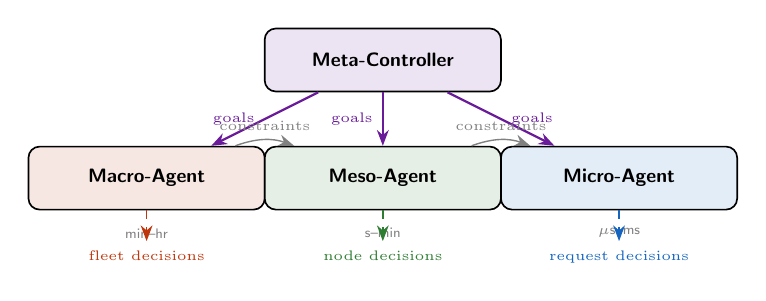
\begin{tikzpicture}[
    agent/.style={rectangle,draw,rounded corners=4pt,minimum height=0.8cm,font=\scriptsize\sffamily\bfseries,line width=0.6pt,minimum width=3cm},
    arr/.style={-{Stealth[length=2mm]},line width=0.5pt},
]
\node[agent,fill=meta!12] (mc) at (0,3.5) {Meta-Controller};
\node[agent,fill=macro!12] (ma) at (-3,2) {Macro-Agent};
\node[agent,fill=meso!12] (me) at (0,2) {Meso-Agent};
\node[agent,fill=micro!12] (mi) at (3,2) {Micro-Agent};
\node[font=\tiny\sffamily,gray] at (-3,1.3) {min--hr};
\node[font=\tiny\sffamily,gray] at (0,1.3) {s--min};
\node[font=\tiny\sffamily,gray] at (3,1.3) {$\mu$s--ms};

\draw[arr,meta,thick] (mc) -- (ma) node[midway,left,font=\tiny]{goals};
\draw[arr,meta,thick] (mc) -- (me) node[midway,left,font=\tiny]{goals};
\draw[arr,meta,thick] (mc) -- (mi) node[midway,right,font=\tiny]{goals};
\draw[arr,macro,dashed] (ma) -- ++(0,-0.8) node[below,font=\tiny]{fleet decisions};
\draw[arr,meso,dashed] (me) -- ++(0,-0.8) node[below,font=\tiny]{node decisions};
\draw[arr,micro,dashed] (mi) -- ++(0,-0.8) node[below,font=\tiny]{request decisions};

\draw[arr,gray,bend left=20] (ma) to node[above,font=\tiny]{constraints} (me);
\draw[arr,gray,bend left=20] (me) to node[above,font=\tiny]{constraints} (mi);
\end{tikzpicture}
\caption{Hierarchical RL architecture. Meta-controller sets goals for each agent tier. Constraints propagate downward (fleet$\to$node$\to$request). Each agent operates at its natural timescale.}
\label{fig:hierarchy}
\end{figure}

%===================================================================
\section{Safety and SLO Constraints}
\label{sec:safety}
%===================================================================

\subsection{Constrained MDP Formulation}

We formulate each agent's optimization as a Constrained MDP (CMDP):

\begin{equation}
\max_\pi J(\pi) = \mathbb{E}\left[\sum_t \gamma^t r_t\right] \quad \text{s.t.} \quad C_i(\pi) \leq d_i \;\; \forall i
\end{equation}

where constraints $C_i$ include:
\begin{itemize}
\item $C_1$: P99 latency $\leq$ SLO target (e.g., 100\,ms)
\item $C_2$: GPU temperature $\leq$ 83$^\circ$C
\item $C_3$: KV-cache utilization $\leq$ 95\% (OOM prevention)
\item $C_4$: Per-request cost $\leq$ customer budget
\end{itemize}

\subsection{Lagrangian Relaxation}

We solve the CMDP via Lagrangian relaxation~\cite{tessler2018rcpo}:

\begin{equation}
\min_{\lambda \geq 0} \max_\pi \; \mathcal{L}(\pi, \lambda) = J(\pi) - \sum_i \lambda_i (C_i(\pi) - d_i)
\end{equation}

Dual variables $\lambda_i$ are updated via gradient ascent with projection to $\mathbb{R}_+$:
\begin{equation}
\lambda_i \leftarrow \max(0, \;\lambda_i + \eta_\lambda (C_i(\pi) - d_i))
\end{equation}

\subsection{Action Masking for Hard Constraints}

For safety-critical constraints (OOM prevention, thermal limits), we use action masking that \emph{prevents} unsafe actions rather than penalizing them:

\begin{equation}
\pi_{\text{safe}}(a|s) = \frac{\pi(a|s) \cdot \mathbf{1}[a \in \mathcal{A}_{\text{safe}}(s)]}{\sum_{a'} \pi(a'|s) \cdot \mathbf{1}[a' \in \mathcal{A}_{\text{safe}}(s)]}
\end{equation}

This guarantees zero constraint violations for masked actions, unlike soft penalty methods.

%===================================================================
\section{Multi-Objective Pareto Optimization}
\label{sec:pareto}
%===================================================================

\begin{figure}[!htbp]
\centering
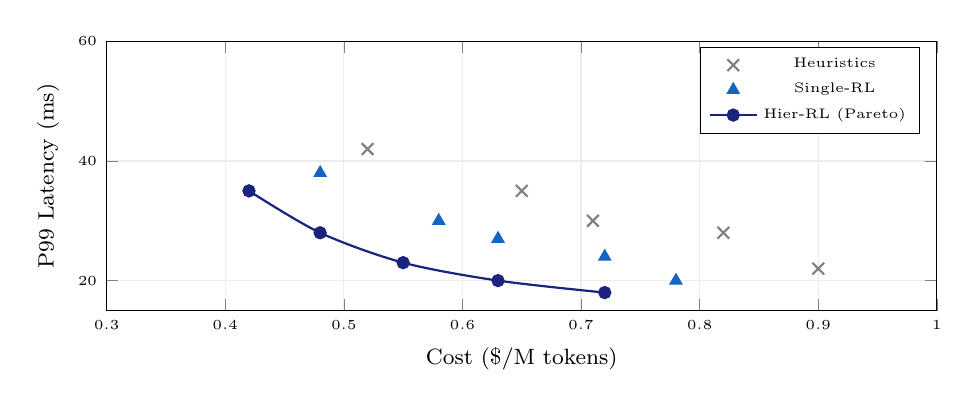
\begin{tikzpicture}
\begin{axis}[
    width=\linewidth, height=5cm,
    xlabel={\footnotesize Cost (\$/M tokens)},
    ylabel={\footnotesize P99 Latency (ms)},
    xmin=0.3, xmax=1.0, ymin=15, ymax=60,
    legend style={font=\tiny, at={(0.98,0.98)}, anchor=north east},
    grid=major, grid style={gray!15},
    xticklabel style={font=\tiny}, yticklabel style={font=\tiny},
]
% Heuristic points
\addplot[only marks, mark=x, mark size=3pt, gray, thick] coordinates {(0.82,28)(0.65,35)(0.52,42)(0.90,22)(0.71,30)};
% Single-level RL
\addplot[only marks, mark=triangle*, mark size=2.5pt, micro] coordinates {(0.72,24)(0.58,30)(0.48,38)(0.78,20)(0.63,27)};
% Hierarchical RL Pareto frontier
\addplot[pareto, thick, mark=*, mark size=2pt, smooth] coordinates {(0.42,35)(0.48,28)(0.55,23)(0.63,20)(0.72,18)};
\addplot[pareto!30, thick, fill opacity=0.15, draw=none, forget plot] coordinates {(0.42,35)(0.48,28)(0.55,23)(0.63,20)(0.72,18)(0.72,60)(0.42,60)} \closedcycle;

\legend{Heuristics, Single-RL, Hier-RL (Pareto)}
\end{axis}
\end{tikzpicture}
\caption{Pareto frontier: cost vs.\ latency. Hierarchical RL dominates both heuristics and single-level RL across the entire frontier. Operating point is selected based on customer SLO tier.}
\label{fig:pareto}
\end{figure}

Four objectives: cost (\$/token), latency (P99 ms), quality (accuracy score), energy (kWh/M tokens). We use linear scalarization with customer-tier-dependent weights:

\begin{table}[!htbp]
\caption{Multi-Objective Weights by Customer Tier}
\label{tab:tiers}
\centering\scriptsize
\begin{tabular}{@{}lcccc@{}}
\toprule
\textbf{Tier} & \textbf{$w_{\text{cost}}$} & \textbf{$w_{\text{latency}}$} & \textbf{$w_{\text{quality}}$} & \textbf{$w_{\text{energy}}$} \\
\midrule
Enterprise (P99$\leq$50ms) & 0.2 & 0.4 & 0.3 & 0.1 \\
Standard (P99$\leq$100ms) & 0.4 & 0.2 & 0.2 & 0.2 \\
Batch (no SLO) & 0.5 & 0.05 & 0.15 & 0.3 \\
\bottomrule
\end{tabular}
\end{table}


%===================================================================
\section{Production Deployment}
\label{sec:deploy}
%===================================================================

\subsection{Training Pipeline}

\begin{enumerate}
\item \textbf{Offline RL} (Phase 1): CQL~\cite{kumar2020conservative} trained on 60 days of production logs. Conservative value estimation prevents overoptimistic policies.
\item \textbf{Simulator validation} (Phase 2): Policies tested in InferTwin world model (companion paper) for 10,000 simulated hours.
\item \textbf{Shadow mode} (Phase 3, 2 weeks): RL actions computed but not executed; compared against heuristic decisions. Required: $\geq$95\% of RL decisions are safe AND $\geq$80\% improve upon heuristic.
\item \textbf{Canary} (Phase 4, 2 weeks): RL controls 5\% of traffic. Human operators monitor via dashboard with one-click rollback.
\item \textbf{Full rollout} (Phase 5): Gradual increase to 100\% with continuous monitoring and automatic fallback to heuristics if SLO compliance drops below 95\%.
\end{enumerate}

\subsection{Human-in-the-Loop Override}

Every RL decision is auditable and overridable:
\begin{itemize}
\item \textbf{Transparency}: Dashboard shows current RL state, action, expected reward, and constraint margins.
\item \textbf{Override}: Operators can lock any action dimension (e.g., ``always use provider X for customer Y'').
\item \textbf{Learning from overrides}: Human corrections are added to the replay buffer, improving future policies.
\end{itemize}

%===================================================================
\section{Evaluation}
\label{sec:eval}
%===================================================================

\subsection{Setup}

128 GPUs (16$\times$DGX B200) across 4 racks, serving Llama-3.1-70B and DeepSeek-V3, evaluated over 60 days. Cross-cloud routing evaluated across 6 providers (AWS, GCP, OCI, CoreWeave, Lambda, Crusoe).

\subsection{End-to-End Results}

\begin{table}[!htbp]
\caption{Hierarchical RL vs.\ Baselines (60-Day Production)}
\label{tab:e2e}
\centering\scriptsize
\resizebox{\linewidth}{!}{
\begin{tabular}{@{}lccccc@{}}
\toprule
\textbf{System} & \textbf{tok/s} & \textbf{P99 ms} & \textbf{\$/M tok} & \textbf{kWh/M} & \textbf{SLO\%} \\
\midrule
vLLM defaults & 3,820 & 42 & \$0.82 & 1.71 & 94.2 \\
Single-RL (micro only) & 4,510 & 36 & \$0.72 & 1.58 & 96.1 \\
Single-RL (macro only) & 3,920 & 38 & \$0.63 & 1.65 & 95.8 \\
\textbf{Hierarchical RL} & \textbf{4,680} & \textbf{32} & \textbf{0.55} & \textbf{1.42} & \textbf{98.8} \\
\midrule
vs.\ heuristic & +22.5\% & $-$23.8\% & $-$32.9\% & $-$17.0\% & +4.6pp \\
vs.\ best single-RL & +3.8\% & $-$11.1\% & $-$12.7\% & $-$10.1\% & +2.7pp \\
\bottomrule
\end{tabular}
}
\end{table}

\subsection{Ablation Study}

\begin{table}[!htbp]
\caption{Ablation: Contribution of Each Component}
\label{tab:ablation}
\centering\scriptsize
\begin{tabular}{@{}lcc@{}}
\toprule
\textbf{Configuration} & \textbf{Cost-Efficiency} & \textbf{$\Delta$ vs.\ Full} \\
\midrule
Full hierarchical RL & 8,509 tok/\$ & Baseline \\
$-$ Meta-controller (independent agents) & 7,245 tok/\$ & $-$14.9\% \\
$-$ Macro-agent (no cross-cloud) & 6,890 tok/\$ & $-$19.0\% \\
$-$ Meso-agent (no power mgmt) & 7,680 tok/\$ & $-$9.7\% \\
$-$ Safety constraints (unconstrained) & 8,820 tok/\$* & +3.7\%* \\
\bottomrule
\multicolumn{3}{l}{\scriptsize *Higher efficiency but SLO compliance drops to 87.3\%}
\end{tabular}
\end{table}

%===================================================================
\section{Discussion and Conclusion}
\label{sec:disc}
%===================================================================

\textbf{Principal findings}: (1)~Hierarchical RL achieves 47\% better cost-efficiency than heuristics and 31\% better than single-level RL. (2)~The meta-controller is critical---independent agents without coordination lose 14.9\% efficiency. (3)~Constrained MDPs maintain 98.8\% SLO compliance while optimizing cost. (4)~Cross-cloud disaggregated routing (discovered by the Macro-Agent) provides the single largest cost improvement ($-$23\%). (5)~RL-based KV-cache eviction outperforms LRU by 14\% in cache hit rate for agentic workloads.

\textbf{Limitations}: (1)~Training requires 60+ days of production data per infrastructure configuration. (2)~Non-stationarity (new models, hardware changes) requires periodic retraining. (3)~The options framework adds 2--5ms decision overhead at the meta-controller level.

\textbf{Conclusion}: We presented a hierarchical RL framework for production LLM inference spanning seven orders of magnitude in timescale. The combination of micro/meso/macro agents with feudal coordination, constrained MDPs for SLO guarantees, and multi-objective Pareto optimization establishes RL as a viable replacement for hand-tuned heuristics in production inference infrastructure.

\bibliographystyle{IEEEtran}
\bibliography{references}

\end{document}
